\documentclass[
  man,
  floatsintext,
  longtable,
  nolmodern,
  notxfonts,
  notimes,
  mask,
  colorlinks=true,linkcolor=blue,citecolor=blue,urlcolor=blue]{apa7}

\usepackage{amsmath}
\usepackage{amssymb}




\RequirePackage{longtable}
% \setlength\LTleft{0pt}
\RequirePackage{threeparttablex}

% % 


\makeatletter
\renewcommand{\paragraph}{\@startsection{paragraph}{4}{\parindent}%
	{0\baselineskip \@plus 0.2ex \@minus 0.2ex}%
	{-.5em}%
	{\normalfont\normalsize\bfseries\typesectitle}}

\renewcommand{\subparagraph}[1]{\@startsection{subparagraph}{5}{0.5em}%
	{0\baselineskip \@plus 0.2ex \@minus 0.2ex}%
	{-\z@\relax}%
	{\normalfont\normalsize\bfseries\itshape\hspace{\parindent}{#1}\textit{\addperi}}{\relax}}
\makeatother




\usepackage{longtable, booktabs, multirow, multicol, colortbl, hhline, caption, array, float}
\setcounter{topnumber}{2}
\setcounter{bottomnumber}{2}
\setcounter{totalnumber}{4}
\renewcommand{\topfraction}{0.85}
\renewcommand{\bottomfraction}{0.85}
\renewcommand{\textfraction}{0.15}
\renewcommand{\floatpagefraction}{0.7}

\usepackage{tcolorbox}
\tcbuselibrary{listings,theorems, breakable, skins}
\usepackage{fontawesome5}

\definecolor{quarto-callout-color}{HTML}{909090}
\definecolor{quarto-callout-note-color}{HTML}{0758E5}
\definecolor{quarto-callout-important-color}{HTML}{CC1914}
\definecolor{quarto-callout-warning-color}{HTML}{EB9113}
\definecolor{quarto-callout-tip-color}{HTML}{00A047}
\definecolor{quarto-callout-caution-color}{HTML}{FC5300}
\definecolor{quarto-callout-color-frame}{HTML}{ACACAC}
\definecolor{quarto-callout-note-color-frame}{HTML}{4582EC}
\definecolor{quarto-callout-important-color-frame}{HTML}{D9534F}
\definecolor{quarto-callout-warning-color-frame}{HTML}{F0AD4E}
\definecolor{quarto-callout-tip-color-frame}{HTML}{02B875}
\definecolor{quarto-callout-caution-color-frame}{HTML}{FD7E14}


% 

\newlength\Oldarrayrulewidth
\newlength\Oldtabcolsep


\usepackage{hyperref}



\usepackage{color}
\usepackage{fancyvrb}
\newcommand{\VerbBar}{|}
\newcommand{\VERB}{\Verb[commandchars=\\\{\}]}
\DefineVerbatimEnvironment{Highlighting}{Verbatim}{commandchars=\\\{\}}
% Add ',fontsize=\small' for more characters per line
\usepackage{framed}
\definecolor{shadecolor}{RGB}{241,243,245}
\newenvironment{Shaded}{\begin{snugshade}}{\end{snugshade}}
\newcommand{\AlertTok}[1]{\textcolor[rgb]{0.68,0.00,0.00}{#1}}
\newcommand{\AnnotationTok}[1]{\textcolor[rgb]{0.37,0.37,0.37}{#1}}
\newcommand{\AttributeTok}[1]{\textcolor[rgb]{0.40,0.45,0.13}{#1}}
\newcommand{\BaseNTok}[1]{\textcolor[rgb]{0.68,0.00,0.00}{#1}}
\newcommand{\BuiltInTok}[1]{\textcolor[rgb]{0.00,0.23,0.31}{#1}}
\newcommand{\CharTok}[1]{\textcolor[rgb]{0.13,0.47,0.30}{#1}}
\newcommand{\CommentTok}[1]{\textcolor[rgb]{0.37,0.37,0.37}{#1}}
\newcommand{\CommentVarTok}[1]{\textcolor[rgb]{0.37,0.37,0.37}{\textit{#1}}}
\newcommand{\ConstantTok}[1]{\textcolor[rgb]{0.56,0.35,0.01}{#1}}
\newcommand{\ControlFlowTok}[1]{\textcolor[rgb]{0.00,0.23,0.31}{\textbf{#1}}}
\newcommand{\DataTypeTok}[1]{\textcolor[rgb]{0.68,0.00,0.00}{#1}}
\newcommand{\DecValTok}[1]{\textcolor[rgb]{0.68,0.00,0.00}{#1}}
\newcommand{\DocumentationTok}[1]{\textcolor[rgb]{0.37,0.37,0.37}{\textit{#1}}}
\newcommand{\ErrorTok}[1]{\textcolor[rgb]{0.68,0.00,0.00}{#1}}
\newcommand{\ExtensionTok}[1]{\textcolor[rgb]{0.00,0.23,0.31}{#1}}
\newcommand{\FloatTok}[1]{\textcolor[rgb]{0.68,0.00,0.00}{#1}}
\newcommand{\FunctionTok}[1]{\textcolor[rgb]{0.28,0.35,0.67}{#1}}
\newcommand{\ImportTok}[1]{\textcolor[rgb]{0.00,0.46,0.62}{#1}}
\newcommand{\InformationTok}[1]{\textcolor[rgb]{0.37,0.37,0.37}{#1}}
\newcommand{\KeywordTok}[1]{\textcolor[rgb]{0.00,0.23,0.31}{\textbf{#1}}}
\newcommand{\NormalTok}[1]{\textcolor[rgb]{0.00,0.23,0.31}{#1}}
\newcommand{\OperatorTok}[1]{\textcolor[rgb]{0.37,0.37,0.37}{#1}}
\newcommand{\OtherTok}[1]{\textcolor[rgb]{0.00,0.23,0.31}{#1}}
\newcommand{\PreprocessorTok}[1]{\textcolor[rgb]{0.68,0.00,0.00}{#1}}
\newcommand{\RegionMarkerTok}[1]{\textcolor[rgb]{0.00,0.23,0.31}{#1}}
\newcommand{\SpecialCharTok}[1]{\textcolor[rgb]{0.37,0.37,0.37}{#1}}
\newcommand{\SpecialStringTok}[1]{\textcolor[rgb]{0.13,0.47,0.30}{#1}}
\newcommand{\StringTok}[1]{\textcolor[rgb]{0.13,0.47,0.30}{#1}}
\newcommand{\VariableTok}[1]{\textcolor[rgb]{0.07,0.07,0.07}{#1}}
\newcommand{\VerbatimStringTok}[1]{\textcolor[rgb]{0.13,0.47,0.30}{#1}}
\newcommand{\WarningTok}[1]{\textcolor[rgb]{0.37,0.37,0.37}{\textit{#1}}}

\providecommand{\tightlist}{%
  \setlength{\itemsep}{0pt}\setlength{\parskip}{0pt}}
\usepackage{longtable,booktabs,array}
\usepackage{calc} % for calculating minipage widths
% Correct order of tables after \paragraph or \subparagraph
\usepackage{etoolbox}
\makeatletter
\patchcmd\longtable{\par}{\if@noskipsec\mbox{}\fi\par}{}{}
\makeatother
% Allow footnotes in longtable head/foot
\IfFileExists{footnotehyper.sty}{\usepackage{footnotehyper}}{\usepackage{footnote}}
\makesavenoteenv{longtable}

\usepackage{graphicx}
\makeatletter
\def\maxwidth{\ifdim\Gin@nat@width>\linewidth\linewidth\else\Gin@nat@width\fi}
\def\maxheight{\ifdim\Gin@nat@height>\textheight\textheight\else\Gin@nat@height\fi}
\makeatother
% Scale images if necessary, so that they will not overflow the page
% margins by default, and it is still possible to overwrite the defaults
% using explicit options in \includegraphics[width, height, ...]{}
\setkeys{Gin}{width=\maxwidth,height=\maxheight,keepaspectratio}
% Set default figure placement to htbp
\makeatletter
\def\fps@figure{htbp}
\makeatother


% definitions for citeproc citations
\NewDocumentCommand\citeproctext{}{}
\NewDocumentCommand\citeproc{mm}{%
  \begingroup\def\citeproctext{#2}\cite{#1}\endgroup}
\makeatletter
 % allow citations to break across lines
 \let\@cite@ofmt\@firstofone
 % avoid brackets around text for \cite:
 \def\@biblabel#1{}
 \def\@cite#1#2{{#1\if@tempswa , #2\fi}}
\makeatother
\newlength{\cslhangindent}
\setlength{\cslhangindent}{1.5em}
\newlength{\csllabelwidth}
\setlength{\csllabelwidth}{3em}
\newenvironment{CSLReferences}[2] % #1 hanging-indent, #2 entry-spacing
 {\begin{list}{}{%
  \setlength{\itemindent}{0pt}
  \setlength{\leftmargin}{0pt}
  \setlength{\parsep}{0pt}
  % turn on hanging indent if param 1 is 1
  \ifodd #1
   \setlength{\leftmargin}{\cslhangindent}
   \setlength{\itemindent}{-1\cslhangindent}
  \fi
  % set entry spacing
  \setlength{\itemsep}{#2\baselineskip}}}
 {\end{list}}
\usepackage{calc}
\newcommand{\CSLBlock}[1]{\hfill\break\parbox[t]{\linewidth}{\strut\ignorespaces#1\strut}}
\newcommand{\CSLLeftMargin}[1]{\parbox[t]{\csllabelwidth}{\strut#1\strut}}
\newcommand{\CSLRightInline}[1]{\parbox[t]{\linewidth - \csllabelwidth}{\strut#1\strut}}
\newcommand{\CSLIndent}[1]{\hspace{\cslhangindent}#1}


\usepackage[nolongtablepatch]{lineno}
\linenumbers


\usepackage{newtx}

\defaultfontfeatures{Scale=MatchLowercase}
\defaultfontfeatures[\rmfamily]{Ligatures=TeX,Scale=1}





\title{APA 7th Edition Template: This is added after the title, no colon
needed.}
\shorttitle{\texttt{shorttitle} is actually the running header.}


\usepackage{etoolbox}


\course{Introduction to Assessment}
\professor{W. Joel Schneider}
\duedate{12/22/2024}




\authorsnames[{1},{2,3}]{
Ryan Straight,Second Author
}




\authorsaffiliations{
{Cyber, Intel, \& Information Operations, University of Arizona},{Second
Author's Primarily Affiliation},{Second Author's Secondary Affiliation}}






\leftheader{Straight and Author}



\abstract{This document is an example of using the \texttt{apaquarto}
extension within the project template. Praesent ornare dolor turpis, sed
tincidunt nisl pretium eget. Curabitur sed iaculis ex, vitae tristique
sapien. Quisque nec ex dolor. Quisque ut nisl a libero egestas molestie.
Nulla vel porta nulla. Phasellus id pretium arcu. Etiam sed mi
pellentesque nibh scelerisque elementum sed at urna. Ut congue molestie
nibh, sit amet pretium ligula consectetur eu. Integer consectetur augue
justo, at placerat erat posuere at. Ut elementum urna lectus, vitae
bibendum neque pulvinar quis. Suspendisse vulputate cursus eros id
maximus. Duis pulvinar facilisis massa, et condimentum est viverra
congue. Curabitur ornare convallis nisl. Morbi dictum scelerisque turpis
quis pellentesque. Etiam lectus risus, luctus lobortis risus ut, rutrum
vulputate justo. Nulla facilisi.}
% 
\keywords{APA, project, template, lipsum}

\authornote{\par{\addORCIDlink{Ryan
Straight}{0000-0002-6251-5662}}\par{\addORCIDlink{Second
Author}{0000-0000-0000-0001}}
\par{ }
\par{       Author roles were classified using the Contributor Role Taxonomy (CRediT; https://credit.niso.org/) as follows: Ryan
Straight:   conceptualization, Writing - original draft; Second
Author:   Formal Analysis, Writing}
\par{Correspondence concerning this article should be addressed to Ryan
Straight, Cyber, Intel, \& Information Operations, University of
Arizona, 1140 N Colombo Ave., Sierra
Vista, AZ 85635, Email: ryanstraight@arizona.edu}
}


\makeatletter
\let\endoldlt\endlongtable
\def\endlongtable{
\hline
\endoldlt
}
\makeatother

\urlstyle{same}





\begin{document}
\maketitle
\setcounter{secnumdepth}{-\maxdimen} % remove section numbering

\setlength\LTleft{0pt}

\resetlinenumber[1]

This is my introductory paragraph. The title will be placed above it
automatically. \emph{Do not start with an introductory heading} (e.g.,
``Introduction''). The title acts as your Level 1 heading for the
introduction. You'll see the
\texttt{\{\{\textless{}\ lipsum\ \textgreater{}\}\}} shortcode used to
flesh out the document. You can add a number to create multiple
paragraphs, like \texttt{\{\{\textless{}\ lipsum\ 3\ \textgreater{}\}\}}
to get three paragraphs. \emph{This requires newer releases of Quarto!}

Duis urna urna, pellentesque eu urna ut, malesuada bibendum dolor.
Suspendisse potenti. Vivamus ornare, arcu quis molestie ultrices, magna
est accumsan augue, auctor vulputate erat quam quis neque. Nullam
scelerisque odio vel ultricies facilisis. Ut porta arcu non magna
sagittis lacinia. Cras ornare vulputate lectus a tristique. Pellentesque
ac arcu congue, rhoncus mi id, dignissim ligula.

Praesent ornare dolor turpis, sed tincidunt nisl pretium eget. Curabitur
sed iaculis ex, vitae tristique sapien. Quisque nec ex dolor. Quisque ut
nisl a libero egestas molestie. Nulla vel porta nulla. Phasellus id
pretium arcu. Etiam sed mi pellentesque nibh scelerisque elementum sed
at urna. Ut congue molestie nibh, sit amet pretium ligula consectetur
eu. Integer consectetur augue justo, at placerat erat posuere at. Ut
elementum urna lectus, vitae bibendum neque pulvinar quis. Suspendisse
vulputate cursus eros id maximus. Duis pulvinar facilisis massa, et
condimentum est viverra congue. Curabitur ornare convallis nisl. Morbi
dictum scelerisque turpis quis pellentesque. Etiam lectus risus, luctus
lobortis risus ut, rutrum vulputate justo. Nulla facilisi.

\subsection{Acronyms}\label{acronyms}

You can add acronyms using the \texttt{acronyms} extension and
shortcodes. For example, \{\{\textless{} acr qmd \textgreater\}\} gives
you Quarto document (qmd). Then, when you use
\{\{\textless{} acr qmd \textgreater\}\} subsequent times, it would
simply show the acronym, like so: qmd. Very convenient. When talking
about qmd frontmatter, you might say:

\begin{quote}
Quarto document (qmd) uses YAML Aint Markup Language (YAML) for
frontmatter, metadata, and settings. YAML is convenient and
human-readable.
\end{quote}

\noindent And the actual text in the file is:

\begin{Shaded}
\begin{Highlighting}[]
\AttributeTok{\textgreater{}\{\{\textless{} acr qmd first\_use=true \textgreater{}\}\} uses \{\{\textless{} acr YAML \textgreater{}\}\} for frontmatter,}
\AttributeTok{metadata, and settings. \{\{\textless{} acr YAML \textgreater{}\}\} is convenient and human{-}readable.}
\end{Highlighting}
\end{Shaded}

\noindent {Note that the code is broken up to wrap in PDF as well as
HTML.} Since we used the \texttt{qmd} acronym in the paragraph above, we
needed to add the \texttt{first\_use=true} option to force the full
acronym usage. You'll also notice the \texttt{\{.NoIndent\}} class
attached to this paragraph and the line above the code block above. Nice
little addition. Readers are better able to follow your ideas if you
differentiate sections in your introduction with headings. Mostly stick
to level 2 headers. Sometimes level 3 headings are needed, though. Be
sparing to the point of stinginess with levels 4 and 5.

All headings should be in title case according to
\href{https://apastyle.apa.org/style-grammar-guidelines/capitalization/title-case}{these
rules and exceptions}.

\subsection{Level 2 Heading}\label{level-2-heading}

Subsections of the introduction have level 2 headings. A paragraph after
a level 2 Heading is on a new line. Regular paragraphs are indented,
flush left, and double-spaced.

You do not need to put text after a heading. You can put a higher-level
heading directly underneath if you want.

Etiam non efficitur urna, quis elementum nisi. Mauris posuere a augue
vel gravida. Praesent luctus erat et ex iaculis interdum. Nulla
vestibulum quam ac nunc consequat vulputate. Nullam iaculis lobortis sem
sit amet fringilla. Aliquam semper, metus ut blandit semper, nulla velit
fermentum sapien, fermentum ultrices dolor sapien sed leo. Vestibulum
molestie faucibus magna, at feugiat nulla ullamcorper a. Aliquam erat
volutpat. Praesent scelerisque magna a justo maximus, sit amet suscipit
mauris tempor. Nulla nec dolor eget ipsum pellentesque lobortis a in
ipsum. Morbi turpis turpis, fringilla a eleifend maximus, viverra nec
neque. Class aptent taciti sociosqu ad litora torquent per conubia
nostra, per inceptos himenaeos.

Duis urna urna, pellentesque eu urna ut, malesuada bibendum dolor.
Suspendisse potenti. Vivamus ornare, arcu quis molestie ultrices, magna
est accumsan augue, auctor vulputate erat quam quis neque. Nullam
scelerisque odio vel ultricies facilisis. Ut porta arcu non magna
sagittis lacinia. Cras ornare vulputate lectus a tristique. Pellentesque
ac arcu congue, rhoncus mi id, dignissim ligula.

\subsection{A Level 2 Heading Without Text Below
It}\label{a-level-2-heading-without-text-below-it}

\subsubsection{Level 3 Heading}\label{level-3-heading}

Subsections of a level 2 heading are placed under level 3 headings.
Vestibulum ultrices, tortor at mattis porta, odio nisi rutrum nulla, sit
amet tincidunt eros quam facilisis tellus. Fusce eleifend lectus in
elementum lacinia. Nam auctor nunc in massa ullamcorper, sit amet auctor
ante accumsan. Nam ut varius metus. Curabitur eget tristique leo. Cras
finibus euismod erat eget elementum. Integer vel placerat ex. Ut id eros
quis lectus lacinia venenatis hendrerit vel ante. Etiam congue quam eget
velit convallis, eu sagittis orci vestibulum. Vestibulum at massa
turpis. Curabitur ornare ex sed purus vulputate, vitae porta augue
rhoncus. Phasellus auctor suscipit purus, vel ultricies nunc. Nunc
eleifend nulla ac purus volutpat, id fringilla felis aliquet. Duis vitae
porttitor nibh, in rhoncus risus. Vestibulum a est vitae est tristique
vehicula. Proin mollis justo id est tempus hendrerit. Praesent suscipit
placerat congue. Aliquam eu elit gravida, consequat augue non, ultricies
sapien. Nunc ultricies viverra ante, sit amet vehicula ante volutpat id.
Etiam tempus purus vitae tellus mollis viverra. Donec at ornare mauris.
Aliquam sodales hendrerit ornare. Suspendisse accumsan lacinia sapien,
sit amet imperdiet dui molestie ut.

\subsubsection{Another Level 3 Heading}\label{another-level-3-heading}

\paragraph{Level 4 Heading.}\label{level-4-heading}

A level 4 heading should be indented, flush left, bold, title case, and
end with a period. A paragraph after a level 4 or 5 heading is on a new
line in this markdown document but will appear as if it were in the same
paragraph when rendered. You need at least one paragraph after a level 4
or 5 heading. If you forget the period at the end of the level 4 or 5
heading, it will be added automatically. A period will not be added if
the heading ends with a question mark or an exclamation point.

Subsequent paragraphs go on their own lines. Etiam non efficitur urna,
quis elementum nisi. Mauris posuere a augue vel gravida. Praesent luctus
erat et ex iaculis interdum. Nulla vestibulum quam ac nunc consequat
vulputate. Nullam iaculis lobortis sem sit amet fringilla. Aliquam
semper, metus ut blandit semper, nulla velit fermentum sapien, fermentum
ultrices dolor sapien sed leo. Vestibulum molestie faucibus magna, at
feugiat nulla ullamcorper a. Aliquam erat volutpat. Praesent scelerisque
magna a justo maximus, sit amet suscipit mauris tempor. Nulla nec dolor
eget ipsum pellentesque lobortis a in ipsum. Morbi turpis turpis,
fringilla a eleifend maximus, viverra nec neque. Class aptent taciti
sociosqu ad litora torquent per conubia nostra, per inceptos himenaeos.
Duis urna urna, pellentesque eu urna ut, malesuada bibendum dolor.
Suspendisse potenti. Vivamus ornare, arcu quis molestie ultrices, magna
est accumsan augue, auctor vulputate erat quam quis neque. Nullam
scelerisque odio vel ultricies facilisis. Ut porta arcu non magna
sagittis lacinia. Cras ornare vulputate lectus a tristique. Pellentesque
ac arcu congue, rhoncus mi id, dignissim ligula.

\subparagraph{Level 5 Heading.}\label{level-5-heading}

A level 5 heading should be indented, flush left, bold italic, title
case, and end with a period. Notice that there was no period after this
level 5 heading in the markdown document, but it does appear in the
rendered document.

Subsequent paragraphs go on their own lines.Etiam non efficitur urna,
quis elementum nisi. Mauris posuere a augue vel gravida. Praesent luctus
erat et ex iaculis interdum. Nulla vestibulum quam ac nunc consequat
vulputate. Nullam iaculis lobortis sem sit amet fringilla. Aliquam
semper, metus ut blandit semper, nulla velit fermentum sapien, fermentum
ultrices dolor sapien sed leo. Vestibulum molestie faucibus magna, at
feugiat nulla ullamcorper a. Aliquam erat volutpat. Praesent scelerisque
magna a justo maximus, sit amet suscipit mauris tempor. Nulla nec dolor
eget ipsum pellentesque lobortis a in ipsum. Morbi turpis turpis,
fringilla a eleifend maximus, viverra nec neque. Class aptent taciti
sociosqu ad litora torquent per conubia nostra, per inceptos himenaeos.
Duis urna urna, pellentesque eu urna ut, malesuada bibendum dolor.
Suspendisse potenti. Vivamus ornare, arcu quis molestie ultrices, magna
est accumsan augue, auctor vulputate erat quam quis neque. Nullam
scelerisque odio vel ultricies facilisis. Ut porta arcu non magna
sagittis lacinia. Cras ornare vulputate lectus a tristique. Pellentesque
ac arcu congue, rhoncus mi id, dignissim ligula.

\subsection{How to Cite References}\label{how-to-cite-references}

I am going to cite a reference here in square brackets (Cameron \&
Trivedi, 2013). This reference was in my bibliography file. Etiam quis
tortor luctus, pellentesque ante a, finibus dolor. Phasellus in nibh et
magna pulvinar malesuada. Ut nisl ex, sagittis at sollicitudin et,
sollicitudin id nunc. In id porta urna. Proin porta dolor dolor, vel
dapibus nisi lacinia in. Pellentesque ante mauris, ornare non euismod a,
fermentum ut sapien. Proin sed vehicula enim. Aliquam tortor odio,
vestibulum vitae odio in, tempor molestie justo. Praesent maximus lacus
nec leo maximus blandit. Maecenas turpis velit, ultricies non elementum
vel, luctus nec nunc. Nulla a diam interdum, faucibus sapien viverra,
finibus metus. Donec non tortor diam. In ut elit aliquet, bibendum sem
et, aliquam tortor. Donec congue, sem at rhoncus ultrices, nunc augue
cursus erat, quis porttitor mauris libero ut ex. Nullam quis leo urna.
Donec faucibus ligula eget pellentesque interdum. Lorem ipsum dolor sit
amet, consectetur adipiscing elit. Aenean rhoncus interdum erat ut
ultricies. Aenean tempus ex non elit suscipit, quis dignissim enim
efficitur. Proin laoreet enim massa, vitae laoreet nulla mollis quis.

\subsubsection{Parenthetical References}\label{parenthetical-references}

Here are some variations on parenthetical citations:

\begin{itemize}
\item
  Page references (or any other suffixes are placed after the reference.
  If you want a comma, you'll need to insert it yourself: (Cameron \&
  Trivedi, 2013, pp. 35--41)
\item
  Prefixes (with or without a comma) are placed before the reference:
  (e.g., Cameron \& Trivedi, 2013).
\item
  2 or more citations separated by a semicolon (Cameron \& Trivedi,
  2013; Cohen et al., 2003). If you need a prefix at the beginning of 2
  or more citations, you will have rearrange the citations so that the
  prefix accompanies the citation that is first alphabetically. That is,
  (e.g., Cameron \& Trivedi, 2013; Cohen et al., 2003), not (Cameron \&
  Trivedi, 2013; e.g., Cohen et al., 2003)
\item
  Any prefixes or suffixes needing a literal semicolon will confuse
  Quarto (actually Pandoc). To make it clear that you need to print a
  semicolon, put a backslash before the semicolon: (FOIL; Cameron \&
  Trivedi, 2013).
\end{itemize}

\subsubsection{In-Text references}\label{in-text-references}

\begin{itemize}
\item
  Cameron and Trivedi (2013) said some interesting things.
\item
  Cohen et al. (2003, pp. 101--103) said specific things on specific
  pages.
\item
  Place the reference's year by itself with a minus sign: (2013)
\end{itemize}

\subsubsection{Masked references}\label{masked-references}

Suppose you want to cite a previous reference of yours, but your
anonymity is supposed to be protected in the review process. You can
``mask'' any citation you wish by setting the \texttt{mask} field in the
metadata yaml to \texttt{true}. Then list all citations that need to be
masked in the \texttt{masked-citations} field as shown in this template.
If the \texttt{mask} field is set to \texttt{false}, they will print as
ususual. Depending if it is an inline or parenthetical citation, will be
listed as ``Masked Citations (n.d)'' or ``(Masked Citations, n.d)''.

I have set two of my publications to be masked. In previous studies,
things were asserted (Masked Author, n.d.). Masked Author (n.d.)
asserted them emphatically.

You can mix masked and unmasked citations (Cohen et al., 2003; Masked
Author, n.d.). Proin sodales neque erat, varius cursus diam tincidunt
sit amet. Etiam scelerisque fringilla nisl eu venenatis. Donec sem
ipsum, scelerisque ac venenatis quis, hendrerit vel mauris. Praesent
semper erat sit amet purus condimentum, sit amet auctor mi feugiat. In
hac habitasse platea dictumst. Nunc ac mauris in massa feugiat bibendum
id in dui. Praesent accumsan urna at lacinia aliquet. Proin ultricies eu
est quis pellentesque. In vel lorem at nisl rhoncus cursus eu quis mi.
In eu rutrum ante, quis placerat justo. Etiam euismod nibh nibh, sed
elementum nunc imperdiet in. Praesent gravida nunc vel odio lacinia, at
tempus nisl placerat. Aenean id ipsum sed est sagittis hendrerit non in
tortor. Lorem ipsum dolor sit amet, consectetur adipiscing elit. Duis
sagittis posuere ligula sit amet lacinia. Duis dignissim pellentesque
magna, rhoncus congue sapien finibus mollis. Ut eu sem laoreet, vehicula
ipsum in, convallis erat. Vestibulum magna sem, blandit pulvinar augue
sit amet, auctor malesuada sapien. Nullam faucibus leo eget eros
hendrerit, non laoreet ipsum lacinia. Curabitur cursus diam elit, non
tempus ante volutpat a. Quisque hendrerit blandit purus non fringilla.
Integer sit amet elit viverra ante dapibus semper. Vestibulum viverra
rutrum enim, at luctus enim posuere eu. Orci varius natoque penatibus et
magnis dis parturient montes, nascetur ridiculus mus.

\subsection{Block Quotes and Suppressing
Indentation}\label{block-quotes-and-suppressing-indentation}

Sometimes you want to give a longer quote that needs to go in its own
paragraph. Block quotes are on their own line starting with the
\texttt{\textgreater{}} character. For example, Jane Austen's
(1814/1990) \emph{Mansfield Park} has some memorable insights about the
mind:

\begin{quote}
If any one faculty of our nature may be called more wonderful than the
rest, I do think it is memory. There seems something more speakingly
incomprehensible in the powers, the failures, the inequalities of
memory, than in any other of our intelligences. The memory is sometimes
so retentive, so serviceable, so obedient; at others, so bewildered and
so weak; and at others again, so tyrannic, so beyond control! We are, to
be sure, a miracle every way; but our powers of recollecting and of
forgetting do seem peculiarly past finding out. (p.~163)
\end{quote}

\noindent If the text after a quote is a new paragraph, you can create
it in the usual fashion (i.e., plain text with an empty line between the
block text and the new paragraph). However, if the text after a quote is
part of the same paragraph, you can suppress the indentation by creating
a div with the .NoIndent class. This paragraph is an example of how to
do so.

\subsection{Hypotheses, Aims, and
Objectives}\label{hypotheses-aims-and-objectives}

The last paragraph of the introduction usually states the specific
hypotheses of the study, often in a way that links them to the research
design.

\section{Method}\label{method}

General remarks on method. This paragraph is optional.

Not all papers require each of these sections. Edit them as needed.
Consult the \href{https://apastyle.apa.org/jars}{Journal Article
Reporting Standards} for what is needed for your type of article.

\subsection{Participants}\label{participants}

Who are they? How were they recruited? Report criteria for participant
inclusion and exclusion. Perhaps some basic demographic stats are in
order. A table is a great way to avoid repetition in statistical
reporting.

\subsection{Measures}\label{measures}

This section can also be titled \textbf{Materials} or
\textbf{Apparatus}. Whatever tools, equipment, or measurement devices
used in the study should be described.

\subsubsection{Measure A}\label{measure-a}

Describe Measure A.

\subsubsection{Measure B}\label{measure-b}

Describe Measure B.

\subsection{Procedure}\label{procedure}

What did participants do?

How are the data going to be analyzed?

\section{Results}\label{results}

\subsection{Descriptive Statistics}\label{descriptive-statistics}

Here we describe the basic characteristics of our primary variables.

\subsection{Displaying Figures}\label{displaying-figures}

Let's make a figure. A reference label for a figure must have the prefix
\texttt{fig-}, and in a code chunk, the caption must be set with
\texttt{fig-cap}.

\phantomsection\label{cell-fig-myplot}
\begin{figure}[H]

{\caption{{This is the figure caption.}{\label{fig-myplot}}}}

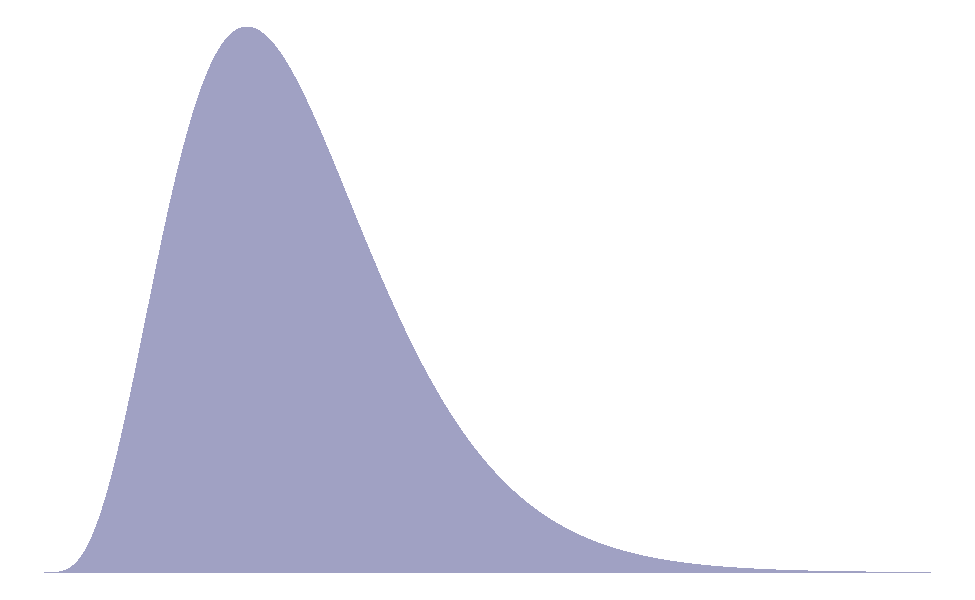
\includegraphics{index_files/figure-pdf/fig-myplot-1.pdf}

{\noindent \emph{Note.} This is the note below the figure.}

\end{figure}

\textsubscript{Source:
\href{https://mavrxlab.github.io/project-template/index.qmd.html}{Article
Notebook}}

To refer to any figure or table, use the \texttt{@} symbol followed by
the reference label, eg., Figure~\ref{fig-myplot}.

\subsection{Updated Syntax for Figures and
Tables}\label{updated-syntax-for-figures-and-tables}

A previous version of this extension used the \texttt{apafg-} prefix for
figure chunk labels and \texttt{apatb-} prefix for tables. It was always
in the plan to use standard Quarto syntax as soon as possible. It is now
possible. Replace all instances of \texttt{apafg-} with the standard
Quarto prefix \texttt{fig-}. Likewise, replace the non-standard
\texttt{apatb-} prefix with the standard Quarto prefix \texttt{tbl-}.

Also replace all text references to figures and tables using standard
Quarto syntax. For example, \texttt{\{apafg-myplot\}} should now be
\texttt{@fig-myplot} instead.

\subsection{Imported Graphics}\label{imported-graphics}

One way to import an existing graphic as a figure is to use
\texttt{knitr::include\_graphics} in a code chunk. For example,
Figure~\ref{fig-importedgraphic} is an imported image. Note that in
apaquarto-pdf documents, we can specify that that a figure or table
should span both columns when in journal mode by setting the
\texttt{apa-twocolumn} chunk option to \texttt{true}. For other formats,
this distinction does not matter.

\phantomsection\label{cell-fig-importedgraphic}
\begin{figure*}[h]

{\caption{{This is an imported graphic.}{\label{fig-importedgraphic}}}}

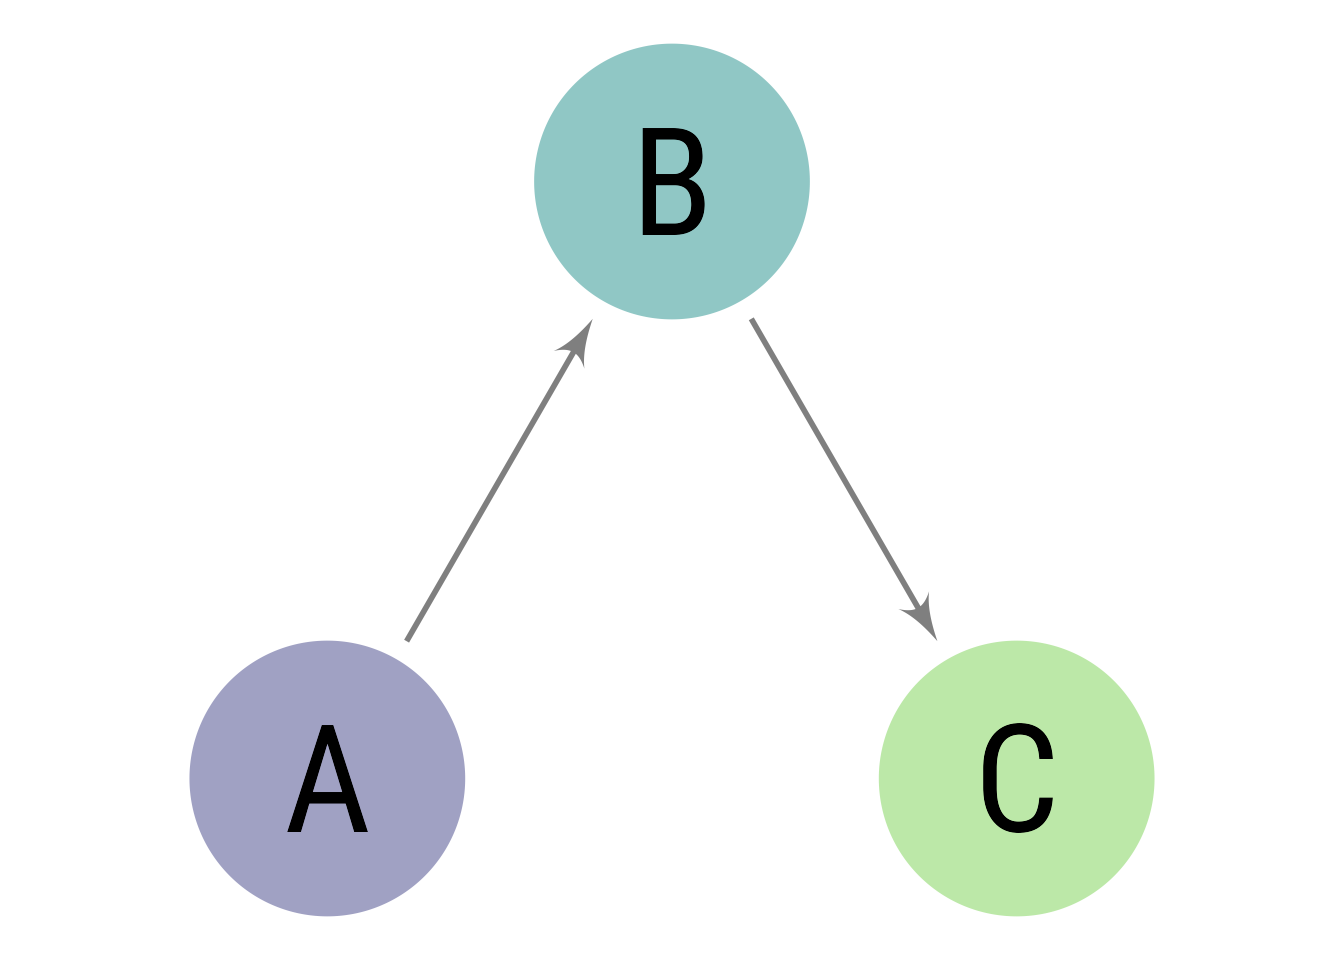
\includegraphics[width=0.5\textwidth,height=\textheight]{4-Outputs/sampleimage.png}

\end{figure*}

\textsubscript{Source:
\href{https://mavrxlab.github.io/project-template/index.qmd.html}{Article
Notebook}}

\subsection{Displaying Tables}\label{displaying-tables}

We can make a table the same way as a figure. Generating a table that
conforms to APA format in all document formats can be tricky. When the
table is simple, the \texttt{kable} function from knitr works well. Feel
free to experiment with different methods, but I have found that David
Gohel's \href{https://davidgohel.github.io/flextable/}{flextable} to be
the best option when I need something more complex.

\begin{table}

{\caption{{Here is the table caption.}{\label{tbl-mytable}}}
\vspace{-20pt}}

\global\setlength{\Oldarrayrulewidth}{\arrayrulewidth}

\global\setlength{\Oldtabcolsep}{\tabcolsep}

\setlength{\tabcolsep}{0pt}

\renewcommand*{\arraystretch}{1.5}



\providecommand{\ascline}[3]{\noalign{\global\arrayrulewidth #1}\arrayrulecolor[HTML]{#2}\cline{#3}}

\begin{longtable*}[l]{|p{0.75in}|p{0.75in}}



\ascline{0.75pt}{000000}{1-2}

\multicolumn{1}{>{\centering}m{\dimexpr 0.75in+0\tabcolsep}}{\textcolor[HTML]{000000}{\fontsize{11}{11}\selectfont{Numbers}}} & \multicolumn{1}{>{\centering}m{\dimexpr 0.75in+0\tabcolsep}}{\textcolor[HTML]{000000}{\fontsize{11}{11}\selectfont{Letters}}} \\

\ascline{0.75pt}{000000}{1-2}\endfirsthead 

\ascline{0.75pt}{000000}{1-2}

\multicolumn{1}{>{\centering}m{\dimexpr 0.75in+0\tabcolsep}}{\textcolor[HTML]{000000}{\fontsize{11}{11}\selectfont{Numbers}}} & \multicolumn{1}{>{\centering}m{\dimexpr 0.75in+0\tabcolsep}}{\textcolor[HTML]{000000}{\fontsize{11}{11}\selectfont{Letters}}} \\

\ascline{0.75pt}{000000}{1-2}\endhead



\multicolumn{1}{>{\centering}m{\dimexpr 0.75in+0\tabcolsep}}{\textcolor[HTML]{000000}{\fontsize{11}{11}\selectfont{1}}} & \multicolumn{1}{>{\centering}m{\dimexpr 0.75in+0\tabcolsep}}{\textcolor[HTML]{000000}{\fontsize{11}{11}\selectfont{A}}} \\





\multicolumn{1}{>{\centering}m{\dimexpr 0.75in+0\tabcolsep}}{\textcolor[HTML]{000000}{\fontsize{11}{11}\selectfont{2}}} & \multicolumn{1}{>{\centering}m{\dimexpr 0.75in+0\tabcolsep}}{\textcolor[HTML]{000000}{\fontsize{11}{11}\selectfont{B}}} \\





\multicolumn{1}{>{\centering}m{\dimexpr 0.75in+0\tabcolsep}}{\textcolor[HTML]{000000}{\fontsize{11}{11}\selectfont{3}}} & \multicolumn{1}{>{\centering}m{\dimexpr 0.75in+0\tabcolsep}}{\textcolor[HTML]{000000}{\fontsize{11}{11}\selectfont{C}}} \\





\multicolumn{1}{>{\centering}m{\dimexpr 0.75in+0\tabcolsep}}{\textcolor[HTML]{000000}{\fontsize{11}{11}\selectfont{4}}} & \multicolumn{1}{>{\centering}m{\dimexpr 0.75in+0\tabcolsep}}{\textcolor[HTML]{000000}{\fontsize{11}{11}\selectfont{D}}} \\

\ascline{0.75pt}{000000}{1-2}



\end{longtable*}



\arrayrulecolor[HTML]{000000}

\global\setlength{\arrayrulewidth}{\Oldarrayrulewidth}

\global\setlength{\tabcolsep}{\Oldtabcolsep}

\renewcommand*{\arraystretch}{1}

{\vspace{-20pt}
\noindent \emph{Note.} Here is the note below the table.}

\end{table}

\textsubscript{Source:
\href{https://mavrxlab.github.io/project-template/index.qmd.html}{Article
Notebook}}

To refer to this table in text, put the table's reference label in curly
braces like so: As seen in Table~\ref{tbl-mytable}, the first few
numbers and letters of the alphabet are displayed.

In Table~\ref{tbl-mymarkdowntable}, there is an example of a plain
markdown table with a note below it.

\begin{table}

{\caption{{Table caption of a markdown
table}{\label{tbl-mymarkdowntable}}}
\vspace{-20pt}}

\begin{longtable}[]{@{}llrc@{}}
\toprule\noalign{}
Default & Left & Right & Center \\
\midrule\noalign{}
\endhead
\bottomrule\noalign{}
\endlastfoot
12 & 12 & 12 & 12 \\
123 & 123 & 123 & 123 \\
1 & 1 & 1 & 1 \\
\end{longtable}

{\vspace{-20pt}
\noindent \emph{Note.} This is a note below the markdown table.}

\end{table}

What if you want the tables and figures to be at the end of the
document? In the .pdf format, you can set the \texttt{floatsintext}
option to false. For .html and .docx documents, there is not yet an
automatic way to put tables and figures at the end. You can, of course,
just put them all at the end, in order. The reference labels will work
no matter where they are in the text.

\section{Discussion}\label{discussion}

Describe results in non-statistical terms. Etiam maximus accumsan
gravida. Maecenas at nunc dignissim, euismod enim ac, bibendum ipsum.
Maecenas vehicula velit in nisl aliquet ultricies. Nam eget massa
interdum, maximus arcu vel, pretium erat. Maecenas sit amet tempor
purus, vitae aliquet nunc. Vivamus cursus urna velit, eleifend dictum
magna laoreet ut. Duis eu erat mollis, blandit magna id, tincidunt
ipsum. Integer massa nibh, commodo eu ex vel, venenatis efficitur
ligula. Integer convallis lacus elit, maximus eleifend lacus ornare ac.
Vestibulum scelerisque viverra urna id lacinia. Vestibulum ante ipsum
primis in faucibus orci luctus et ultrices posuere cubilia curae; Aenean
eget enim at diam bibendum tincidunt eu non purus. Nullam id magna
ultrices, sodales metus viverra, tempus turpis. Duis ornare ex ac
iaculis pretium. Maecenas sagittis odio id erat pharetra, sit amet
consectetur quam sollicitudin. Vivamus pharetra quam purus, nec sagittis
risus pretium at. Nullam feugiat, turpis ac accumsan interdum, sem
tellus blandit neque, id vulputate diam quam semper nisl. Donec sit amet
enim at neque porttitor aliquet. Phasellus facilisis nulla eget placerat
eleifend. Vestibulum non egestas eros, eget lobortis ipsum. Nulla rutrum
massa eget enim aliquam, id porttitor erat luctus. Nunc sagittis quis
eros eu sagittis. Pellentesque dictum, erat at pellentesque
sollicitudin, justo augue pulvinar metus, quis rutrum est mi nec felis.
Vestibulum efficitur mi lorem, at elementum purus tincidunt a. Aliquam
finibus enim magna, vitae pellentesque erat faucibus at. Nulla mauris
tellus, imperdiet id lobortis et, dignissim condimentum ipsum. Morbi
nulla orci, varius at aliquet sed, facilisis id tortor. Donec ut urna
nisi.

\subsection{Limitations and Future
Directions}\label{limitations-and-future-directions}

Every study has limitations. Based on this study, some additional steps
might include\ldots{} Etiam congue quam eget velit convallis, eu
sagittis orci vestibulum. Vestibulum at massa turpis. Curabitur ornare
ex sed purus vulputate, vitae porta augue rhoncus. Phasellus auctor
suscipit purus, vel ultricies nunc. Nunc eleifend nulla ac purus
volutpat, id fringilla felis aliquet. Duis vitae porttitor nibh, in
rhoncus risus. Vestibulum a est vitae est tristique vehicula. Proin
mollis justo id est tempus hendrerit. Praesent suscipit placerat congue.
Aliquam eu elit gravida, consequat augue non, ultricies sapien. Nunc
ultricies viverra ante, sit amet vehicula ante volutpat id. Etiam tempus
purus vitae tellus mollis viverra. Donec at ornare mauris. Aliquam
sodales hendrerit ornare. Suspendisse accumsan lacinia sapien, sit amet
imperdiet dui molestie ut. Etiam non efficitur urna, quis elementum
nisi. Mauris posuere a augue vel gravida. Praesent luctus erat et ex
iaculis interdum. Nulla vestibulum quam ac nunc consequat vulputate.
Nullam iaculis lobortis sem sit amet fringilla. Aliquam semper, metus ut
blandit semper, nulla velit fermentum sapien, fermentum ultrices dolor
sapien sed leo. Vestibulum molestie faucibus magna, at feugiat nulla
ullamcorper a. Aliquam erat volutpat. Praesent scelerisque magna a justo
maximus, sit amet suscipit mauris tempor. Nulla nec dolor eget ipsum
pellentesque lobortis a in ipsum. Morbi turpis turpis, fringilla a
eleifend maximus, viverra nec neque. Class aptent taciti sociosqu ad
litora torquent per conubia nostra, per inceptos himenaeos.

\subsection{Conclusion}\label{conclusion}

Let's sum this up. Nunc ac dignissim magna. Vestibulum vitae egestas
elit. Proin feugiat leo quis ante condimentum, eu ornare mauris feugiat.
Pellentesque habitant morbi tristique senectus et netus et malesuada
fames ac turpis egestas. Mauris cursus laoreet ex, dignissim bibendum
est posuere iaculis. Suspendisse et maximus elit. In fringilla gravida
ornare. Aenean id lectus pulvinar, sagittis felis nec, rutrum risus. Nam
vel neque eu arcu blandit fringilla et in quam. Aliquam luctus est sit
amet vestibulum eleifend. Phasellus elementum sagittis molestie. Proin
tempor lorem arcu, at condimentum purus volutpat eu. Fusce et
pellentesque ligula. Pellentesque id tellus at erat luctus fringilla.
Suspendisse potenti. Etiam maximus accumsan gravida. Maecenas at nunc
dignissim, euismod enim ac, bibendum ipsum. Maecenas vehicula velit in
nisl aliquet ultricies. Nam eget massa interdum, maximus arcu vel,
pretium erat. Maecenas sit amet tempor purus, vitae aliquet nunc.
Vivamus cursus urna velit, eleifend dictum magna laoreet ut. Duis eu
erat mollis, blandit magna id, tincidunt ipsum. Integer massa nibh,
commodo eu ex vel, venenatis efficitur ligula. Integer convallis lacus
elit, maximus eleifend lacus ornare ac. Vestibulum scelerisque viverra
urna id lacinia. Vestibulum ante ipsum primis in faucibus orci luctus et
ultrices posuere cubilia curae; Aenean eget enim at diam bibendum
tincidunt eu non purus. Nullam id magna ultrices, sodales metus viverra,
tempus turpis.

\newpage

\section{References}\label{references}

\phantomsection\label{refs}
\begin{CSLReferences}{1}{0}
\bibitem[\citeproctext]{ref-austenMansfieldPark1990}
Austen, J. (1990). \emph{Mansfield {P}ark}. Oxford University Press.
(Original work published 1814)

\bibitem[\citeproctext]{ref-CameronTrivedi2013}
Cameron, A. C., \& Trivedi, P. K. (2013). \emph{Regression analysis of
count data} (2nd ed.). Cambridge University Press.
\url{https://doi.org/10.1017/CBO9781139013567}

\bibitem[\citeproctext]{ref-cohen2003applied}
Cohen, J., Cohen, P., West, S. G., \& Aiken, L. S. (2003). \emph{Applied
multiple regression/correlation analysis for the behavioral sciences}
(3rd ed.). Lawrence Erlbaum Associates.

\bibitem[\citeproctext]{ref-maskedreference}
Masked Author. (n.d.). \emph{Masked Title}.

\end{CSLReferences}

\newpage

\section{Appendix A: List of
Acronyms}\label{appendix-a-list-of-acronyms}

\begin{description}
\tightlist
\item[\phantomsection\label{acronyms_qmd}{qmd}]
Quarto document
\item[\phantomsection\label{acronyms_YAML}{YAML}]
YAML Aint Markup Language
\end{description}





\end{document}
